\chapter{Opdracht 2: Use cases en domeinmodel}

\section{Stap 1: Analyseer de use cases van blackjack}
We hebben de opdracht doorgenomen en weten wat de opdrachtgever van ons verwacht.

We moeten ons voorstellen hoe blackjack precies werkt in de echte wereld.
Daarvan willen we een model maken in diagrammen en code, maar ook in ons hoofd!

Laten we een use case diagram maken, zodat de acties die door het systeem
aangeboden moeten worden voldoende duidelijk zijn. Hiervoor kan je het use case 
diagram van Figuur~\ref{fig:chips-use-cases} als inspiratie nemen.

\begin{figure}[H]
    \centering
    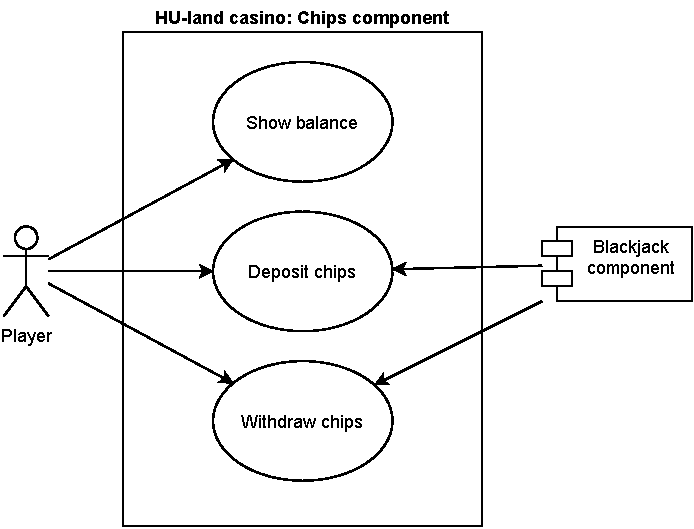
\includegraphics[height=0.4\linewidth]{chips-use-cases}
    \caption{De use cases van het chips-component}
    \label{fig:chips-use-cases}
\end{figure}

Neem de opdrachtbeschrijving door en denk na over de volgende zaken:
\begin{enumerate}
    \item Welke actors zijn er? Geautomatiseerde actors hoef je niet op te nemen.
    \item Wat wordt er binnen het component allemaal afgehandeld? Dit zijn geen use cases!
    \item Welke use cases moeten er naar buiten toe aangeboden worden om blackjack te kunnen spelen?
\end{enumerate}

Gebruik een tool als \textit{diagrams.net}, \textit{software ideas modeler} of \textit{visual paradigm},
sla het ontwerp op en exporteer het als \textit{.png} of \textit{.jpg}. 
Neem dit op in je projectdirectory (bijvoorbeeld onder een mapje \textit{diagrams}),
zodat je docent er naar kan kijken en er feedback op kan geven.

Commit je wijzigingen met een duidelijke naam, 
bijvoorbeeld: "Add use case diagram for blackjack". 
Push de wijzigingen naar je remote GitHub repository.

\section{Het objectmodel}
Wanneer je werkt met objecten, is het goed om het objectmodel van Booch in 
het achterhoofd te houden.\footnote{
    In de praktijk wordt ook wel eens verwezen naar de \texit{4 Pillars of Object Orientation}: 
    abstraction, encapsulation, polymorphism en inheritance. 
    Deze zijn in het objectmodel van Booch inbegrepen.
}

Het objectmodel van Booch onderscheidt vier belangrijke elementen 
die een rol spelen bij het object-georiënteerd modelleren:
\begin{enumerate}
    \item Abstraction
    \item Encapsulation 
    \item Modularity 
    \item Hierarchy
\end{enumerate}

Deze onderdelen noemen Booch et al. belangrijk omdat je 
zonder deze elementen geen object-georiënteerde taal (OO-taal) kan hebben.
Daarnaast beschrijven zij drie minder belangrijke elementen die je 
bij veel OO-talen tegen kunt komen: typing, persistence en concurrency.

Dit betekent natuurlijk niet dat je deze zaken buiten OO-talen niet tegen zal komen! 

\newpage
Het objectmodel van Booch onderscheid een aantal zaken
die ons helpen goed gestructureerde object-georiënteerde software te ontwerpen.

Dit komt tijdens de colleges aan bod, maar kunnen we als volgt samenvatten:
\begin{enumerate}
    \item \textbf{Abstraction}: klassen en objecten zijn onze kernabstracties waarin we 
    toestand (fields) en gedrag (methods) samenbrengen die bij elkaar horen. Dit verhoogt \textit{cohesion}.
    We kunnen met deze abstracties communiceren via de publieke methoden. 
    De interne werking hoeven we dan niet te weten (\textit{implementation hiding}).
    \item \textbf{Encapsulation}: hoe een abstractie zijn toestand bijhoudt en zijn 
    gedrag uitvoert wordt afgeschermd van de buitenwereld. Om \textit{information hiding} te bereiken wordt 
    gebruik gemaakt van access modifiers (bijvoorbeeld: \textit{private}). 
    Dit beperkt \textit{coupling}. Wees spaarzaam met getters en setters (\textit{Tell, don't Ask}) 
    en wees niet afhankelijk van de onderdelen binnen een klasse \textit(\textit{Law of Demeter}).
    \item \textbf{Modularity}: klassen zijn modules waarin we toestand en gedrag samenbrengen. Daarnaast kennen 
    we interfaces om bepaald gedrag af te dwingen en enums om mogelijke waarden op te sommen. 
    Packages kunnen we gebruiken om klassen en andere modules te ordenen.
    \item \textbf{Hierarchy}: we kunnen packages onderbrengen in een logische, overzichtelijke ordening. Dat is onderdeel 
    van een softwarearchitectuur. Ook klassen en objecten kunnen in een hiërarchie tot elkaar staan. Er zijn namelijk 
    verschillende afhankelijkheden die tussen klassen kan gelden: \textit{dependency}, \textit{association}, \textit{aggregation},
    \textit{composition}, \textit{inheritance} en \textit{realisation}. Wat betreft inheritance en realisation zorgen 
    \textit{subtyping}, \textit{polymorphism} en \textit{dynamic binding} ervoor dat we een flexibele, uitwisselbare 
    invulling kunnen hebben van bepaalde abstracties. Eén abstractie kan namelijk verschillende vormen aannemen tijdens runtime:
    een subtype kan een implementatie of overschrijving verzorgen van het supertype.
\end{enumerate}

\newpage
\section{Stap 2: Ontwerp een globaal domeinmodel}
Zodra je hebt nagedacht over de use cases en hier een model van hebt gemaakt,
kunnen we een overzicht maken van de concepten die we nodig hebben in ons blackjack-component.

Hiervoor kunnen we een versimpeld domeinmodel maken. 
Methods, attributes, rolnamen en multipliciteiten mag je achterwege laten.
Wees niet bang om veel concepten te modelleren!

Loop nogmaals door de opdrachtbeschrijving en verwerk de volgende zaken in je 
domeinmodel:
\begin{enumerate}
    \item Welke concepten leven er in de wereld van blackjack? 
    \item Wat zijn goede kandidaten voor klassen en enums?
    \item Wat zijn de relaties tussen deze concepten? Geef dit aan met de juiste pijlen.
    \item Welk concept kunnen we als centraal aanspreekpunt aanmerken waar we andere concepten aan kunnen hangen?
\end{enumerate}

Probeer hier niet teveel tijd aan te besteden.
Dit is een eerste opzet om het domein te structureren.
Tijdens het programmeren leren we meer over het domein, de functionaliteit en de structuur
en gaan we dit nader invullen en aanpassen!

Gebruik een tool als \textit{diagrams.net}, \textit{software ideas modeler} of \textit{visual paradigm},
sla het ontwerp op en exporteer het als \textit{.png} of \textit{.jpg}. 
Neem dit op in je projectdirectory (bijvoorbeeld onder een mapje \textit{diagrams}),
zodat je docent er naar kan kijken en er feedback op kan geven.

Commit je wijzigingen met een duidelijke naam, 
bijvoorbeeld: "Design initial domain model for blackjack". 
Push de wijzigingen naar je remote GitHub repository.

De docent geeft algemene of specifieke feedback
op basis waarvan je je domeinmodel kunt verbeteren.
Wat we alvast kunnen weggeven is dat je een spelpotje 
als centrale domeinklasse kan nemen.

\newpage
\section{Stap 3: Realiseer eerste domeinconcepten}
Het kan handig zijn om met deze stap te beginnen als je al wat feedback hebt 
gehad op je domeinmodel, maar je kan natuurlijk alvast beginnen en het na 
de feedback verbeteren.

We gaan de basis van ons domein leggen door alvast wat klassen aan te maken.
De methodes kunnen we nu al toevoegen, maar dit kunnen we ook later doen. 
Alvast een tip: probeer nog geen getters of setters te maken. 
Setters heb je meestal niet nodig en getters maken we pas aan wanneer
we de data daadwerkelijk uit een object moeten halen. Dit is eigenlijk alleen 
het geval wanneer je een soort vertaalslag moet uitvoeren, bijvoorbeeld tussen 
lagen of tussen ons systeem en de buitenwereld.

Laten we eerst weer de IDE induiken en beginnen met packages aan te maken!
Deze packages hebben een betekenisvolle rol in onze architectuur: 
we willen separation of concerns, high cohesion en loose coupling.

\subsection{Maak packages}
In IntelliJ kan je packages aanmaken door met de rechtermuisknop op de package
in het projectoverzicht (links) te klikken waar je iets nieuws wil toevoegen
en dan naar \texttt{New > Package} te gaan 
(je kan ook `package' typen of de pijltjestoetsen gebruiken). 
Als alternatief kan je ook de parent-package selecteren en dan 
het generate-scherm openen met \texttt{ALT + INSERT} (MacOS: \texttt{COMMAND + N}). 

Maak een nieuwe package aan: \texttt{nl.hu.bep2.casino.blackjack}.
Dit is de package voor ons component, ons deelgebied, dat over blackjack zal gaan.
We zijn bezig met het modelleren van het domein. Laten we daarvoor een laag aanmaken.
Ook daarvoor maken we een package: \texttt{nl.hu.bep2.casino.blackjack.domain}.

In deze package zouden we nog subpackages kunnen aanmaken, bijvoorbeeld om zaken te groeperen.
Denk bijvoorbeeld aan concepten die herbruikbaar zijn voor allerlei soorten kaartspellen 
in plaats van alleen voor blackjack. Dan zouden we een package kunnen aanmaken: 
\\ \texttt{nl.hu.bep2.casino.blackjack.domain.cards}. Dit kunnen we ook doen zodra we 
wat verder zijn en bekend is welke concepten er in ons domein leven.

Let op: packagenamen schrijven we in Java altijd met kleine letters,
zonder leestekens!

\subsection{Voeg klassen en enums toe}
Laten we beginnen met één centrale klasse dat ons aanspreekpunt wordt
voor domeinacties. Die klasse wordt ook het uitgangspunt wanneer we het gaan opslaan.

Maak deze centrale klasse aan. Selecteer in het projectoverzicht de 
package waaraan je een klasse wil toevoegen en klik rechtermuisknop, \texttt{New > Class}. 
Ook hier kan je hotkeys gebruiken: \texttt{ALT + INSERT} (MacOS: \texttt{COMMAND + N}).
Laten we het een Engelse naam geven dat spelpotje betekent (bijvoorbeeld: \texttt{Game} of \texttt{Table}).

Let op: klasse-, interface, en enum-namen schrijven we in Java altijd met in Pascal-case 
(\textit{StudlyCaps}), zonder leestekens!

Wat moet een spelpotje allemaal gaan bijhouden? Probeer dit op te nemen in de fields.
We willen bijvoorbeeld het huidige pakje speelkaarten bijhouden voor dit spelpotje.
Zorg dan dat je klasse er als volgt uit ziet. Vraag je af: waarom declareren we dit veld als \textit{private}?

\begin{minted}{java}
    package nl.hu.bep2.casino.blackjack.domain;

    public class Game {
        private Deck deck;
    }
\end{minted}

Als het goed is, is \texttt{Deck} in IntelliJ roodgekleurd 
of voorzien van een waarschuwing. Leer dit soort signalen te herkennen!
Om de \texttt{Deck} aan te maken, kan je met je cursor (of caret) op de het
type gaan staan (\texttt{Deck}) en de klasse laten genereren door de hotkeys
\texttt{ALT + ENTER} (MacOS: \texttt{OPTION + ENTER}) te gebruiken 
(show intention actions). Selecteer `create class' en geef de package aan 
waar je de klasse in wil aanmaken. Druk op \texttt{ENTER}.

\subsection{Vul de rest van de objectboom in}
Voeg vervolgens op deze zelfde manier alle andere velden (en de bijbehorende klassen) toe 
die deze centrale \texttt{Game}-klasse nodig heeft.
Voeg ook de velden toe van de velden van deze klasse en herhaal dit proces totdat
je je objectboom klaar hebt.

Je zou \texttt{Deck} kunnen voorzien van een verzameling van kaarten 
en een kaart weer van een rang en een kleur. Denk na over hoe je rang en kleur en 
handigst in Java kunt programmeren op een leesbare en herbruikbare manier.
Er is een manier die ervoor zorgt dat je nooit een kaart kan maken met een niet-bestaande 
rang of kleur. Er zijn maar 52 mogelijkheden: 4 kleuren en 13 rangen.

Je mag ook al methodes aanmaken, maar het gaat ons nu vooral om een eerste structuur.
We weten pas hoe de methodes precies werken zodra we onze use cases implementeren 
in een applicatie service (zie volgende opdracht).

Commit je wijzigingen met een duidelijke naam, 
bijvoorbeeld: "Structure initial domain concepts". 
Push de wijzigingen naar je remote GitHub repository.

\subsection{Maak constructors aan}
Maak voor elke klasse in ons domein een constructor aan.
Een constructor is een speciaal soort (statische) methode die wordt aangeroepen
om een objectinstantie te maken. Daar kunnen we ook instanties aan meegeven om 
de velden te vullen.

Ook constructors kan je genereren. Zet je cursor op een veld en klik 
rechtermuisknop `Show Context Actions' of gebruik de hotkey \texttt{ALT + ENTER} 
(MacOS: \texttt{OPTION + ENTER}) terwijl je caret op een veld staat. 
Je kan ook willekeurig op een plek in je klasse je caret neerzetten en iets genereren 
met \texttt{ALT + INSERT} (MacOS: \texttt{OPTION + N}).

Nu opent er een scherm om een constructor te genereren op basis van de velden. Je kan 
gemakkelijk alle velden selecteren door \texttt{SHIFT} ingedrukt te houden en 
pijltje naarbeneden te doen totdat je alle velden geselecteerd hebt. Vervolgens kan je 
op \texttt{ENTER} drukken om je keuze te bevestigen. Dan krijg je nog wat opties om de 
constructor aan te passen, maar meestal hoeft dat niet. Druk nogmaals op \texttt{ENTER}.

\begin{minted}{java}
    package nl.hu.bep2.casino.blackjack.domain.cards;

    public class Deck {
        private List<Card> cards;

        public Deck(List<Card> cards) {
            this.cards = cards;
        }
    }
\end{minted}

Je kan ook waarden initialiseren in de velden zelf. Dan hoef je ze niet mee te geven 
in de constructor, maar heeft een veld een bepaalde startwaarde wanneer een object 
geïnitialiseerd wordt. Denk bijvoorbeeld aan een lijst van kaarten, zoals in een Deck.
Als je met een lege Deck wil beginnen kan je het volgende doen:

\begin{minted}{java}
    package nl.hu.bep2.casino.blackjack.domain.cards;

    public class Deck {
        private List<Card> cards = new ArrayList<>();
    }
\end{minted}

Wil je een nieuw veld toevoegen aan een bestaande constructor? Declareer dan eerst het veld
en ga vervolgens met je caret op dit (grijze) veld staan. 
Doe wederom \texttt{ALT + ENTER} (MacOS: \texttt{OPTION + ENTER})
en kies `Add constructor parameter'.

Commit je wijzigingen met een duidelijke naam, 
bijvoorbeeld: ``Add constructors to domain concepts''. 
Push de wijzigingen naar je remote GitHub repository.

\subsection{Tip: een named constructor toevoegen aan Deck}
Beginnen met een lege Deck en van buitenaf allerlei kaarten toevoegen 
(bijvoorbeeld in de constructor of een \texttt{add(Card card)} methode)
is misschien niet de meest praktische oplossing.

Waarschijnlijk willen we elke keer als we een nieuwe Deck maken
deze vullen met kaarten. Daarvoor kunnen we een zogenaamde \textit{named constructor}
maken: een static method op \texttt{Deck} die een \texttt{Deck} teruggeeft 
na alle kaarten toegevoegd te hebben. Om een volle deck terug te geven, zouden 
we een functie met de volgende vorm kunnen aanmaken:

\begin{minted}{java}
public class Deck {
    private List<Card> cards = new ArrayList<>();

    public static Deck full() {
        Deck deck = new Deck();

        // TODO: Creation of all cards and adding them to the deck

        return deck;
    }
}
\end{minted}

Binnen de \texttt{full}-methode kunnen we kaarten toevoegen aan de 
deck-instantie door \texttt{deck.cards.add(card)} te doen. De \texttt{card}
moet je dan wel zelf aanmaken.

Hoe je precies de kaarten moet aanmaken en toevoegen aan de Deck,
laten we nog even aan jou. Afhankelijk van hoe je de kaarten gemodelleerd hebt 
in je spel, kan je dit oplossen zonder alle 52 kaarten met de hand te benoemen!

\subsection{Voeg al wat methods toe}
Het is goed om alvast wat gedrag toevoegen aan de objecten!
Maar wees niet bang om ze later aan te passen of te verwijderen.
Overbodige code is dode code.

Naast welke objecten precies welke verantwoordelijkheid hebben 
kunnen we ook nadenken over het gedrag dat zij aanbieden; 
het domein is meer dan slechts met getters en setters data heen en weer te schuiven. 
Een algemene tip is om te denken in gedrag in plaats van data. 
Setters heb je eigenlijk bijna niet nodig, getters alleen wanneer je ze aanroept. 

Probeer het object op zichzelf te beschouwen: welke vragen (queries) zou je eraan willen stellen? 
Welke acties (commands) zou je het willen laten uitvoeren? 
Waar bestaat het object uit en moet het object met andere objecten samenwerken? 
Andere objecten waarmee samengewerkt wordt, afhankelijkheden, 
kunnen we het beste in de constructor meegeven of als parameter van de methode die wordt aangeroepen. 
Het doel is om te komen tot een goed georganiseerde objectstructuur met één duidelijk aanspreekpunt: 
een game object dat later kan worden opgeslagen. 
Dit game object heeft kennis van allerlei onderliggende domeinconcepten 
die elk hun eigen specifieke verantwoordelijkheid hebben. 
Wees niet bang om veel objecten aan te maken met kleine methodes per specifieke actie! 
Ook hier komen de eigenschappen van het objectmodel om de hoek kijken.

Je kan je klassen testen door gebruik te maken van JUnit of het even 
in een Main-functie uit te proberen. We gaan het later handmatig testen met 
Postman. In een latere cursus gaan we dieper op het correct testen van object-georiënteerde projecten in.

\subsection{Tip: Gebruik je IDE!}
Wil je een klasse of package verplaatsen, versleep deze dan in het projectoverzicht.
Alle imports en verwijzingen worden automatisch geupdate. Wil je hiervoor een hotkey gebruiken,
dan is dat \texttt{F6} (MacOS: \texttt{F6}) terwijl je het betreffende item hebt geselecteerd 
in het projectoverzicht of open hebt staan in de editor. Je kan ook gebruik maken van 
het refactor-menu door rechtermuisknop op een klasse of package te doen.

Wil je een klasse of package hernoemen, dan kan je rechtermuisknop 
\texttt{Refactor > Rename} doen of de hotkeys \texttt{SHIFT + F6} (MacOS: SHIFT + F6).
Dezelfde hotkey kan je gebruiken om velden, variabelen en methoden te hernoemen.

Gebruik voor dit soort zaken altijd je IDE! Dit bespaart je een hoop tijd omdat je IDE 
het op allerlei plekken tegelijkertijd voor je aanpast. Op het hele project kan slim gebruik 
van je IDE je uren besparen! 

Er zijn nog meer van dit soort hotkeys. 
Voor een overzicht, zie: \href{https://www.jetbrains.com/help/idea/reference-keymap-win-default.html}{Windows hotkeys} 
of \href{https://www.jetbrains.com/help/idea/reference-keymap-mac-default.html}{MacOS hotkeys}.

Heb je geen zin om steeds de handleiding of Google te gebruiken? Dan kan je altijd de hotkey 
\texttt{CTRL + SHIFT + A} gebruiken om een trefwoord te typen van wat je wil doen.
Vaak geeft IntelliJ een goede suggestie. 

Wil je geïnformeerd worden wanneer je iets doet waar je een hotkey voor had kunnen gebruiken?
Dan kan je de IntelliJ-plugin Keypromotor X installeren, zie 
\href{https://www.jetbrains.com/help/idea/mastering-keyboard-shortcuts.html#learn-shortcuts}{IntelliJ's uitleg}.
